\documentclass[review]{elsarticle}

\usepackage{lineno,hyperref}
\modulolinenumbers[5]


% Prettify tables
\usepackage{tabularx, booktabs, float, pbox, rotating, caption}
% Create new column type - centred X
\newcolumntype{C}{>{\centering\arraybackslash}X} 

% For inputting graphics
\usepackage{graphicx}
% Define path
\graphicspath{ {./figures/} }
% Rotating pages
\usepackage{pdflscape}

\usepackage[modulo]{lineno}
\linenumbers
\modulolinenumbers[1]

%% `Elsevier LaTeX' style
\bibliographystyle{elsarticle-num}
%%%%%%%%%%%%%%%%%%%%%%%

% Define journal name
\journal{Computers, Environment and Urban Systems}

% Begin doc
\begin{document}
	
\setlength{\parskip}{\baselineskip}
\setlength{\parindent}{0pt}

% Begin frontmater
\begin{frontmatter}
	% Define paper title 
	\title{Identifying urban areas: A new approach and comparison of national urban metrics with gridded population data}
	% Define author info
	\author[Affil1]{Thomas Statham\corref{cor1}}
	\ead{thomas.statham@bristol.ac.uk}
	\author[Affil1]{Sean Fox}
	\ead{sean.fox@bristol.ac.uk}
	\author[Affil1]{Levi John Wolf}
	\ead{levi.john.wolf@bristol.ac.uk}
	\address[Affil1]{School of Geographical Sciences, University of Bristol, University Road, Bristol, BS8 1SS, United Kingdom}
	\cortext[cor1]{Corresponding Author: Thomas Statham, School of Geographical Sciences, University of Bristol, University Road, Bristol, BS8 1SS, United Kingdom; Email, thomas.statham@bristol.ac.uk; Phone, +44 (0)117 928 9954}
		
\begin{abstract}			
	The measurement of urbanization and other key urban indicators depends on how urban areas are defined.
	The Degree of Urbanization (DEGURBA) has been recently adopted to support international statistical comparability, but its rigid criteria for classify areas as urban/non-urban based upon fixed population size and density criteria is controversial.
	Here we present an alternative approach to urban classification, using a flexible range of population density \& count thresholds.
	We then compare how these thresholds affect estimation of urbanization and urban settlement counts across three of the most popular gridded population datasets (GPD).
	Instead of introducing further uncertainties by matching GPD to built-up area datasets, we classify urban areas in a purely spatial demographic way.
	By calculating national urban shares and urban area counts, we highlight the often overlooked uncertainties when using GPD.
	We find that the choice of GPD is generally the dominant factor in altering both of these urban indicators but the choice of urban criteria is also important.
	Overall, this alternative urban classification method offers a more
	flexible approach to human settlements classification that can be applied globally for comparative research.
	
\end{abstract}
\begin{keyword}
	\sep Urban classification \sep Gridded population datasets  \sep Urbanization \sep Urban areas
\end{keyword}

\end{frontmatter}

	
	\newpageafter{abstract}
	
	\section{Introduction}
	On March 5th 2020, the United Nations (UN) Statistical Commission agreed on a global, harmonized definition for measuring the ``Degree of Urbanization'' (DEGURBA) across member states for the very first time \cite{UN2020}.
	This newly agreed definition is based on prior work undertaken by the European Union (EU) to create a common classification system for human settlements across member states.
	Adopting the DEGURBA classification system facilitates global comparison and monitoring of UN Sustainable Development Goals.
	In addition, a growing body of research has adopted the DEGURBA definition, 
	including examining urban carbon footprints \cite{Moranetal2018}, green urban areas \cite{Corbaneetal2018}, mapping travel times to urban centres globally \cite{Weissetal2018} and modelling global urban street networks \cite{Boeing2021}.
	Overall, the DEGURBA is becoming increasingly integrated into both urban policy and research, which has the potential to shape the future of urban areas.
	
	
	Prior to this agreement, international statistical comparisons of urban indicators were undermined by the fact every country has a unique set of criteria for classifying human settlements and the statistical geographies used for classification are drawn arbitrarily, to achieve a minimum population size \cite{Foxetal2017}.
	This is problematic because classified statistical geographies rarely align exactly with regions considered to be urban areas, which limits their validity when making international statistical comparisons \cite{Buettner2015, Taubenboecketal2017}.
	The DEGURBA methodology instead applies standardised criteria for identifying settlements into three classes; cities, peri-urban areas and rural areas, expressed as regular, gridded geographies.
	The DEGURBA draws on two harmonised EU datasets: the Global Human Settlement Population (GHS-POP) and GHS Settlement Model (SMOD), which are classified based on population size, population counts and built-up area densities. 
	Whilst the classification of urban areas using standardised geographies and urban definitions does facilitate international statistical comparisons, the rigid classification criteria has been controversial \cite{Angeletal2019,Ondaetal2019}.
	More generally and related to the above, smaller urban areas are more difficult to classify than larger urban areas using rigid criteria.
	This is reflected by the greater consistency in classification criteria for larger urban areas between countries.
	Consequently, some have argued whether a single urban definition is feasible or even desirable \cite{Saladin2016}.
	
	
	In this paper we propose a more flexible approach to urban classification, which can be customised by researchers or statistical agencies to support a diverse range of applications. 
	Similar to the DEGURBA, we also classify urban areas based on population density and count thresholds but we classify urban areas in a purely spatial demographic way, leveraging the idea that urban areas represent demographically large, densely populated areas \cite{Foxetal2017}.
	This also avoids introducing uncertainties when matching population data to built-up area datasets \cite{Dijkstra2020}.
	Furthermore, we do not use rigid threshold rules but consider a range of urban criteria, as well as several Gridded Population Datasets (GPD).
	This flexibility allows international comparisons but also enables customization on a case by case basis.
	We selected population density and count thresholds based on the range of census-based urban criteria used for classification.
	We applied this to commonly referenced GPDs in the literature: the Gridded Population of the World (GPW) \cite{GPW2016}, GHS-POP \cite{GHSPOP2019} and WorldPop \cite{WorldPop2018} datasets. 
	To assess how the range of urban criteria and choice of GPD affects our understanding of patterns of urbanization, we calculated and compared national urban shares - the percentage of population that resides in urban areas, and urban area counts for several countries.
	We find that the choice of GPD and urban criteria can have a major influence on urbanization estimates.
	When considering population count thresholds in addition to density thresholds for national urban settlement counts, we found that the calculated counts for each GPD was stratified by the choice of population count threshold.
	Additionally, small and medium urban areas are more sensitive to the choice of urban criteria than large urban areas.
	Future research should provide a similar comparison at the global scale to confirm these patterns and more generally, assess GPD against the ground truth.
	
	
	\section{Methods}
	The main aim of this paper is to provide an alternative urban classification methodology to the Degree of Urbanization (DEGURBA).
	Instead of using rigid urban criteria, we adopt a more flexible approach that allows for a wide range of urban shapes, sizes and densities. 
	Prior to outlining our approach, we first describe two alternative approaches to urban classification; census-based and methods that classify the built-up environment or more generally, geographic entities within them.
	
	
	\subsection{Alternative approaches to urban classification}
	Census agencies often classify statistical units for administrative purposes.
	Without clearly defined urban boundaries, resources may be disproportionally allocated, which may in turn exacerbate inequalities \cite{He2018}.
	The most common criteria used to classify urban geographies are minimum population counts \& density thresholds, administrative status and employment composition \cite{Satterthwaite2007, Batty2018}. 
	Population density thresholds are the most commonly used, with 85 countries applying threshold rules that classify any space as urban that has between 200 and 5000 persons per km$^2$ \cite{OECD2020}.
	Whilst census-based urban classifications are useful for understanding socio-economic geographies within countries, statistical comparisons between countries are problematic because of these differences in definitions and statistical units.
	Statistical units are arbitrarily defined for administrative purposes, to achieve a minimum population size \cite{Foxetal2017}. 
	This means that they also rarely align with regions which we consider to be urban areas, so classified urban areas may also include rural areas \cite{Buettner2015, Taubenboecketal2017}.
	
	
	Another set of methods classify city land according to the built environment.
	Whereas census-based urban classifications are place-based, these methods are space-based.
	Early attempts focussed solely on mapping the built environment using low-spatial resolution day-time \cite{Schneider2012, Arinoetal2012} and night-time remotely sensed imagery \cite{Balketal2006}.
	Whilst these methods allowed urban areas to be identified in a standardised way, sensor limitations resulted in high error rates.
	Furthermore, the identification of built-up areas does not necessarily mean the identification of urban areas, where populations reside.
	More recent classifications have focussed on alternative datasets, including commuting patterns \cite{FarmerFotheringham2011, Guéroisetal2014, ShenBatty2019}, building densities \cite{ArribasBeletal2019, Bellefonetal2019} and mobile phone data \cite{Thomasetal2012}.
	Whilst classifying these datasets result in fewer rates of false classifications, these datasets are limited to countries with the ability to collect, store and analyse these datasets.
	Overall, more recent methods that classify the built-up environment are suitable for making statistical comparisons within countries but not for comparing international statistical.
	
	
	The proposed population-based method combines the strength of these two alternative approaches to urban classification.
	Applying readily available GPD allows us to classify urban areas in a standardised way and using a range of urban criteria and GPD enables customization on a case by case basis.
	This flexibility allows researchers or statistical agencies to compare key urban measures at the international scale for a diverse range of applications. 
	
	
	\subsection{Study areas and data} 
	We classified and identified urban areas for 12 countries (Figure \ref{fig:study_areas}). 
	These countries represent a range of income groups and are distributed across several continents.
	
	
	\begin{figure}[H]
		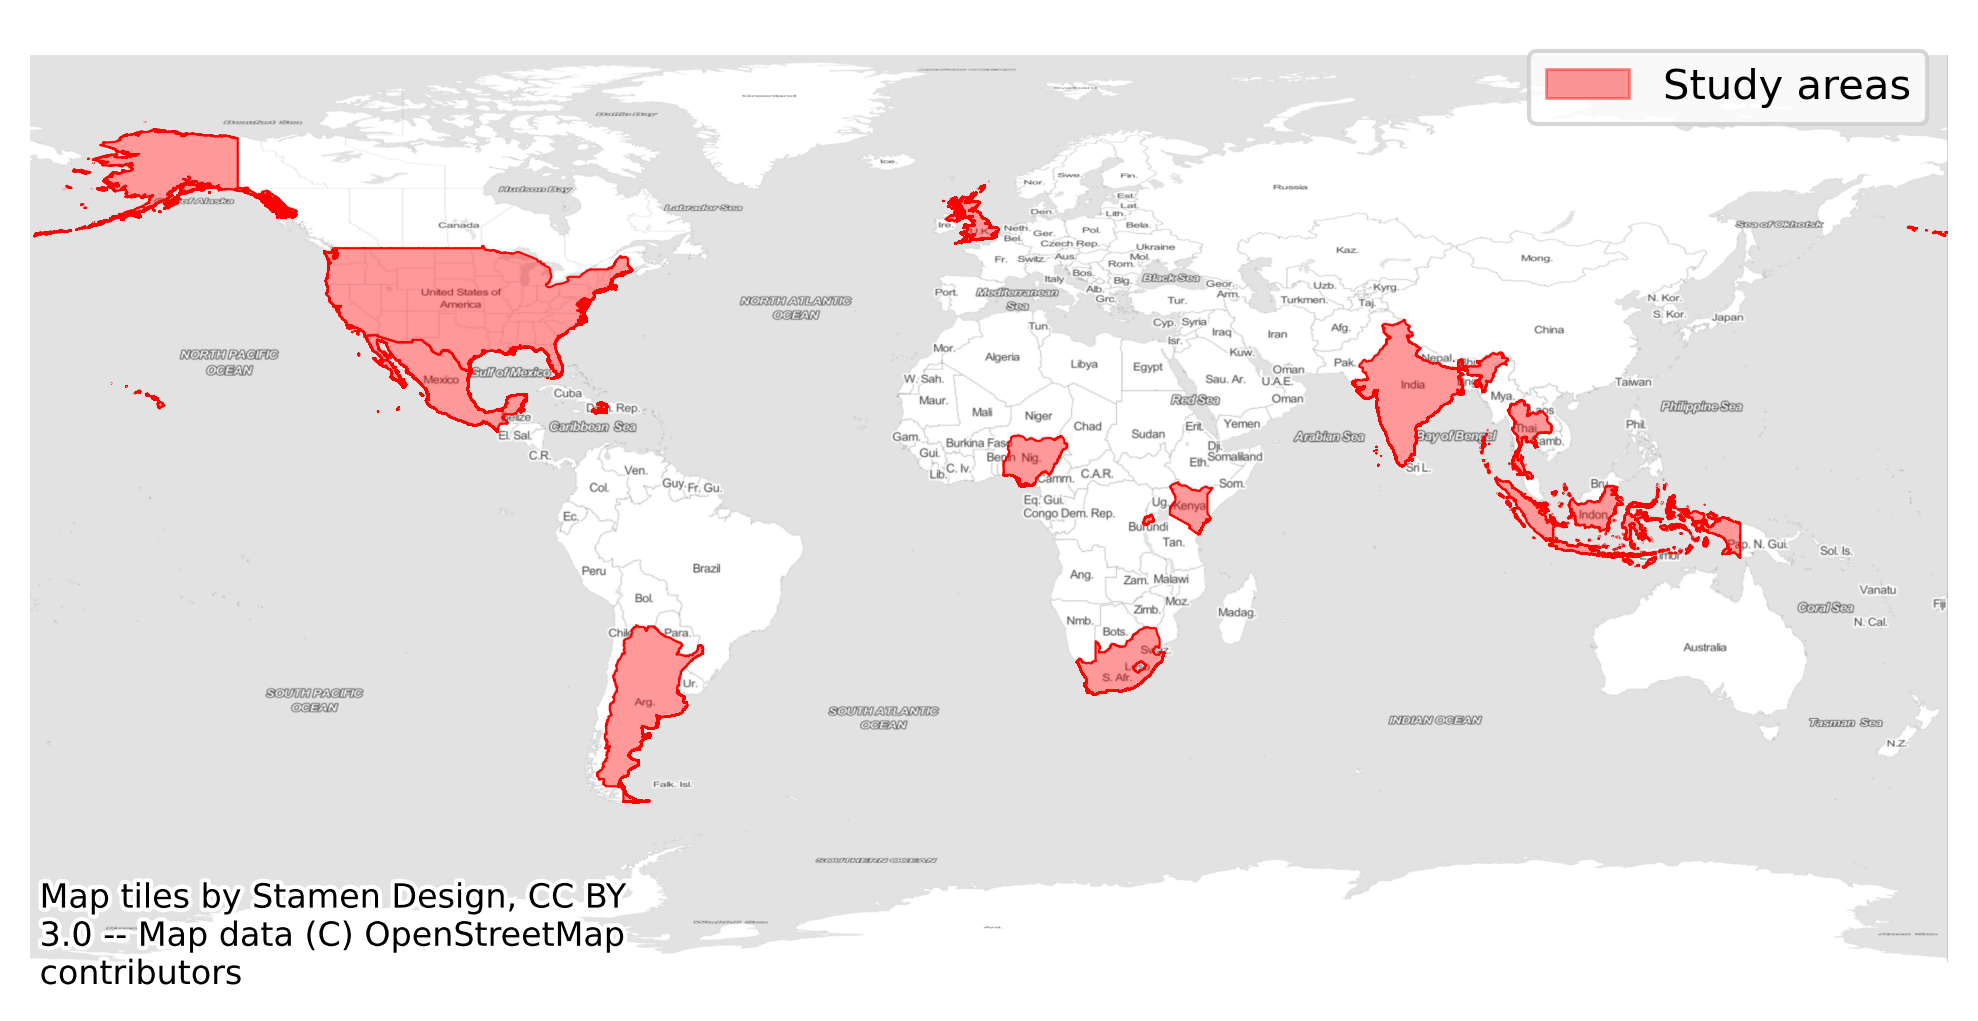
\includegraphics[width=\textwidth]{study_areas}
		\caption{Study areas}
		\label{fig:study_areas}
	\end{figure}
	
	
	We used three GPDs for urban classification; Gridded Population of the World (GPW), Global Human Settlement Population (GHS-POP), and WorldPop datasets.
	Each of these GPD are generated through different areal interpolation methods, so represent a unique population distribution.
	Each areal interpolation method considers different modelling assumptions and some include ancillary data to refine the interpolation.
	These GPD are the most commonly referenced in the literature and any differences between GPDs will highlight their often overlooked uncertainties.
	To make the datasets comparable, we considered adjusted population counts for the year 2015 \footnote{adjusted population counts accounts for any inconsistencies in sources, which can be influenced by factors such as war or corruption}.
	
	
	\subsection{Urban criteria thresholds}
	Our approach allows for a range of population density and count thresholds to be used for human settlement classification.
	This range was determined by common criteria used in census-based urban classification systems.
	We selected population density thresholds ranging from 200 to 4000 persons per km$^2$ in increments of 200 and minimum population requirements of 2500, 5000 and 10000, as well as non minimum per urban area.
	
	
	\subsection{Data processing}
	A 1km$^2$ vector grid was selected to classify urban areas in a consistent way.
	This allows us to compare between GPD and use a range of other urban indicators at this spatial scale or above.
	This was created by vectorizing the same spatial zoning system used by the GHS-POP and GPW datasets \footnote{Cells were clipped using national boundaries, to spatially constrain the population counts within national boundaries. This avoids overcounting when aggregating the gridded population datasets}
	After generating the 1km$^2$ vector grid, each of the gridded population datasets was aggregated and summed using areal-weighted overlay \footnote{This heavy computation was accomplished using the fast and exact zonal statistics implementation Exactextract \cite{Exactextract2020}.
		Other zoning statistics implementations often sacrifice accuracy for performance by not accounting for partial overlaps and instead assume that each raster cell follows an inclusion/exclusion rule relative to the polygons.
		Not accounting for partial overlaps would yield unsatisfactory results.}.
	
	
	\subsection{Classifying and identifying urban areas}
	Classifying grid cells and identifying urban areas was based on the following conditions:
	
	\begin{enumerate}
		\item a grid cell must have a minimum population density criteria to be considered urban; 
		\item if an urban grid cell is ``geographically close'' to another neighbouring urban unit, they merge into the same urban area \footnote{Any remaining cells that are not considered ``geographically close'' to other urban grid cells are still considered urban but exist as single cells};
		\item the total population count of an urban area must also be above a minimum size.
	\end{enumerate}
	
	To satisfy the first condition, we filter out cells that do not match the specified density threshold.
	The second condition is motivated by the assumption that urban areas are densely populated regions separated by sparsely populated regions.
	Using density-based clustering, we group urban cells into clusters that represent urban areas that are similar to each other and dissimilar to other cells.
	The third condition is met by summing the population count of individual urban cells and filtering urban areas which do not meet the total population count threshold.
	
	We apply the well-known density-based clustering algorithm, Density-Based Spatial Clustering of Applications with Noise (DBSCAN) for urban classification \cite{Esteretal1996}. 
	Unlike other density-based methods, it features the well-defined ``density-reachability'' model, which is based on connecting points within a certain distance threshold that also satisfy a density criterion. 
	All other points that lie outside of high-density regions are considered noise.
	This method uses two hyperparameters. 
	The first is $\varepsilon$, which represents the radius or minimum distance of a neighbouring observed object.
	The second is the minimum number of objects or points in the $\varepsilon$ neighbourhood of an observed object (MinPts).
	Let $P$ represent a set of multi-dimensional objects and let the $\varepsilon$-neighbours of an object $p_i$ $\in$ $P$ be $N_{\varepsilon} (p_i)$, DBSCAN considers two rules; 
	An object $p_i$ is an $\varepsilon$-core object if $∣ \ N_{\varepsilon} (p_i) ∣ \ \geq$ MinPts;
	If $p_i$ is an $\varepsilon$-core object, all objects in $∣ \ N_{\varepsilon} (p_i)$ should appear in the same cluster as $p_i$.
	Using this notation, the DBSCAN algorithm can be decomposed into three stages \cite{Schubertetal2017};
	\begin{enumerate}
		\item Find the points ($p_i$) in the $\varepsilon$ neighbourhood of every point ($P$), and identify the core points ($\varepsilon$-core) greater than MinPts neighbours;
		\item Find the connected components of core points ($\varepsilon$-core) on the neighbour graph, ignoring all non-core points;
		\item Assign each non-core point to a nearby cluster if the cluster is an $\varepsilon$ neighbour, otherwise assign it to noise. 
	\end{enumerate}
	
	We consider the neighbourhood graph in a purely data-driven way, based on the distribution of features and motive for clustering.
	In this problem, the motive of clustering is to assign each filtered grid cell to an urban area.
	To assign each filtered urban cell to a cluster, we set the minimum number of points (MinPts) hyperparameter to 1 so that every filtered grid cell belongs to a cluster and no cells are considered noise.
	In other words, all other cells that are filtered out are considered rural.
	Given that geometric centroids are nearly evenly spaced (separated by about 1km 
	at the equator), we set the distance between grid cells in the feature space to 1km.	
	Using the same hyperparameters for every urban grid cell means that each urban boundary is solely based on the choice of population density \& count threshold and GPD.
	
	In comparison to our approach, the EU definition considers contiguity-based clustering to classify urban cells.
	Instead of using a ``density-reachability'' model to specify the neighbourhood graph, contiguity-based clustering can only merge if they are neighbours that share a common border.
	The main consideration when applying contiguity-based clustering is the selection of criterion for the specifying the neighbourhood graph.
	However, this is often arbitrarily selected with little regard to the distribution of features.
	The DEGURBA selects different neighbourhood rules for different settlement typologies \cite{OECD2020} but the choice of criterion for each typology is not well documented.
	The choice of criterion will considerably alter the number of neighbouring grid cells, where the number of neighbours according to the queen criterion will be at least as large as the rook or bishop criterion \cite{Anselin2002}.
	Therefore, the choice of criterion will alter both the shapes and sizes of urban areas.
	
	
	Figure \ref{fig:explaining_method} summarises our flexible urban classification methodology for Bristol and its surrounding areas.
	Part A shows the WorldPop GPD, where darker red shades represent populated areas.  
	Part B shows the 1km$^2$ gridded zoning system.
	Zonal statistics are then applied for each GPD and the generated vector grid, to aggregate and sum each GPD to the same spatial zoning system.  
	In Part C, grid cells are first filtered using density thresholds and then the centroid of each grid cell is clustered using DBSCAN.
	Finally, clustered grid cell groups are aggregated into urban settlements in Part D.
	If a population count threshold is also considered, those urban settlements that do not meet the threshold are dropped.
	This process is repeated for each combination of population density \& population count threshold and GPD.
	
	
	\begin{figure}[H]
		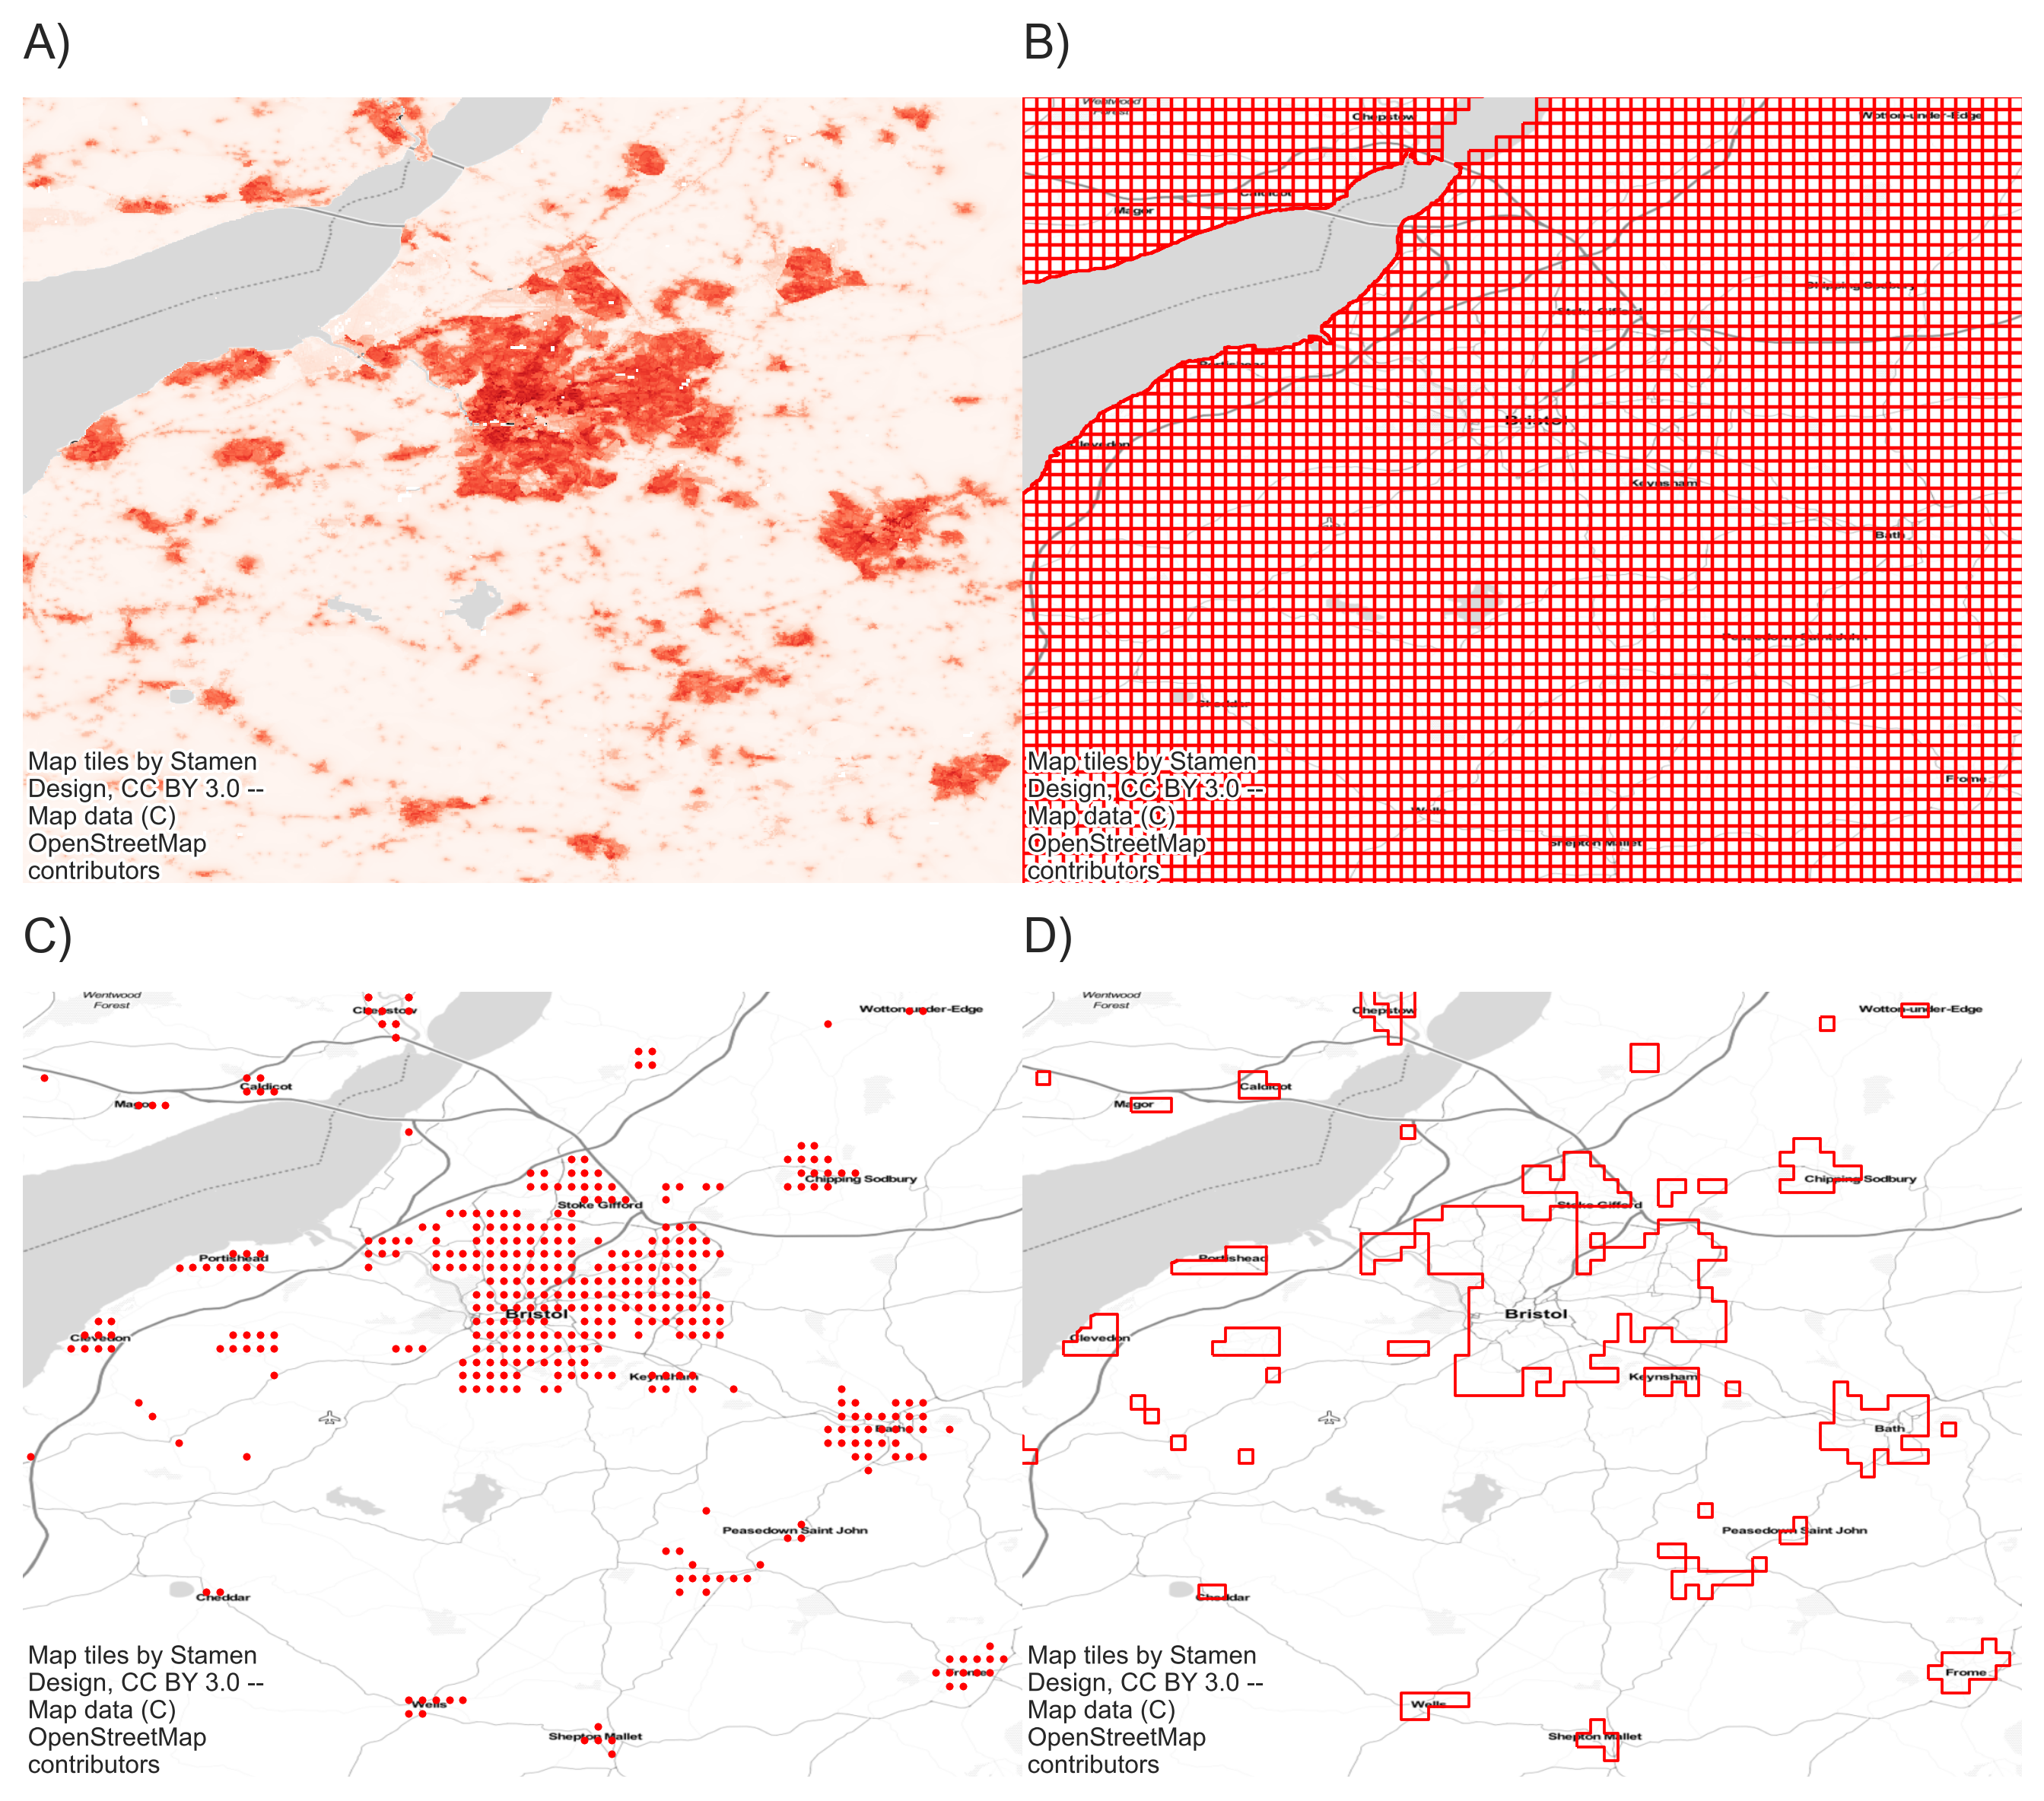
\includegraphics[width=\textwidth]{workflow_bristol}
		\caption{Identifying urban area workflow for Bristol, United Kingdom and surrounding areas: (A) WorldPop Gridded population dataset, (B) Vectorization of gridded population dataset and zonal statistics (C) Classifying cells using threshold rules and clustering methods (D) Dissolving grid cells based on clustered groups}
		\label{fig:explaining_method}
	\end{figure}
	
	
	\subsection{Urban indicators}
	In this study, we calculate two urban indicators; national urban shares and urban area counts. 
	We focus on these two indicators as measures of urbanization and urban expansion.
	Understanding the relationship between these two measures at this scale is important for proportionally allocating international aid, as well as understanding the global diversity of urban form.
	We considered population density thresholds for national urban shares and national urban area counts while varying both population density and count thresholds.
	To directly examine differences between the calculated urban indicators using each urban boundary, we present simple to interpret descriptive statistics.
	
	
	\section{Results}
	We assess the different urban classification criteria and GPD by comparing the calculated national urban shares and urban area counts for each case study.
	Before comparing the urban indicators for each case study, we illustrate our urban classification methodology for a single case study, using several density thresholds.
	
	\subsection{Total land area and urban shapes}
	\label{S:urban_shapes}
	
	Using the WorldPop dataset, we classify urban areas using several density thresholds for Haiti (Figure \ref{fig:hti_worldpop_explain_method}).
	For each successive density threshold, there is an expected decrease in total land area covered by urban areas because fewer grid cells are classified as urban.
	Given our methodology is a strictly spatial demographic approach, it stands that as the total land area covered by urban areas decreases, urbanization will also decrease.
	We will assess the total range of density thresholds considered by comparing national shares and urban area counts in Section \ref{S:nus}.
	
	\begin{figure}[H]
		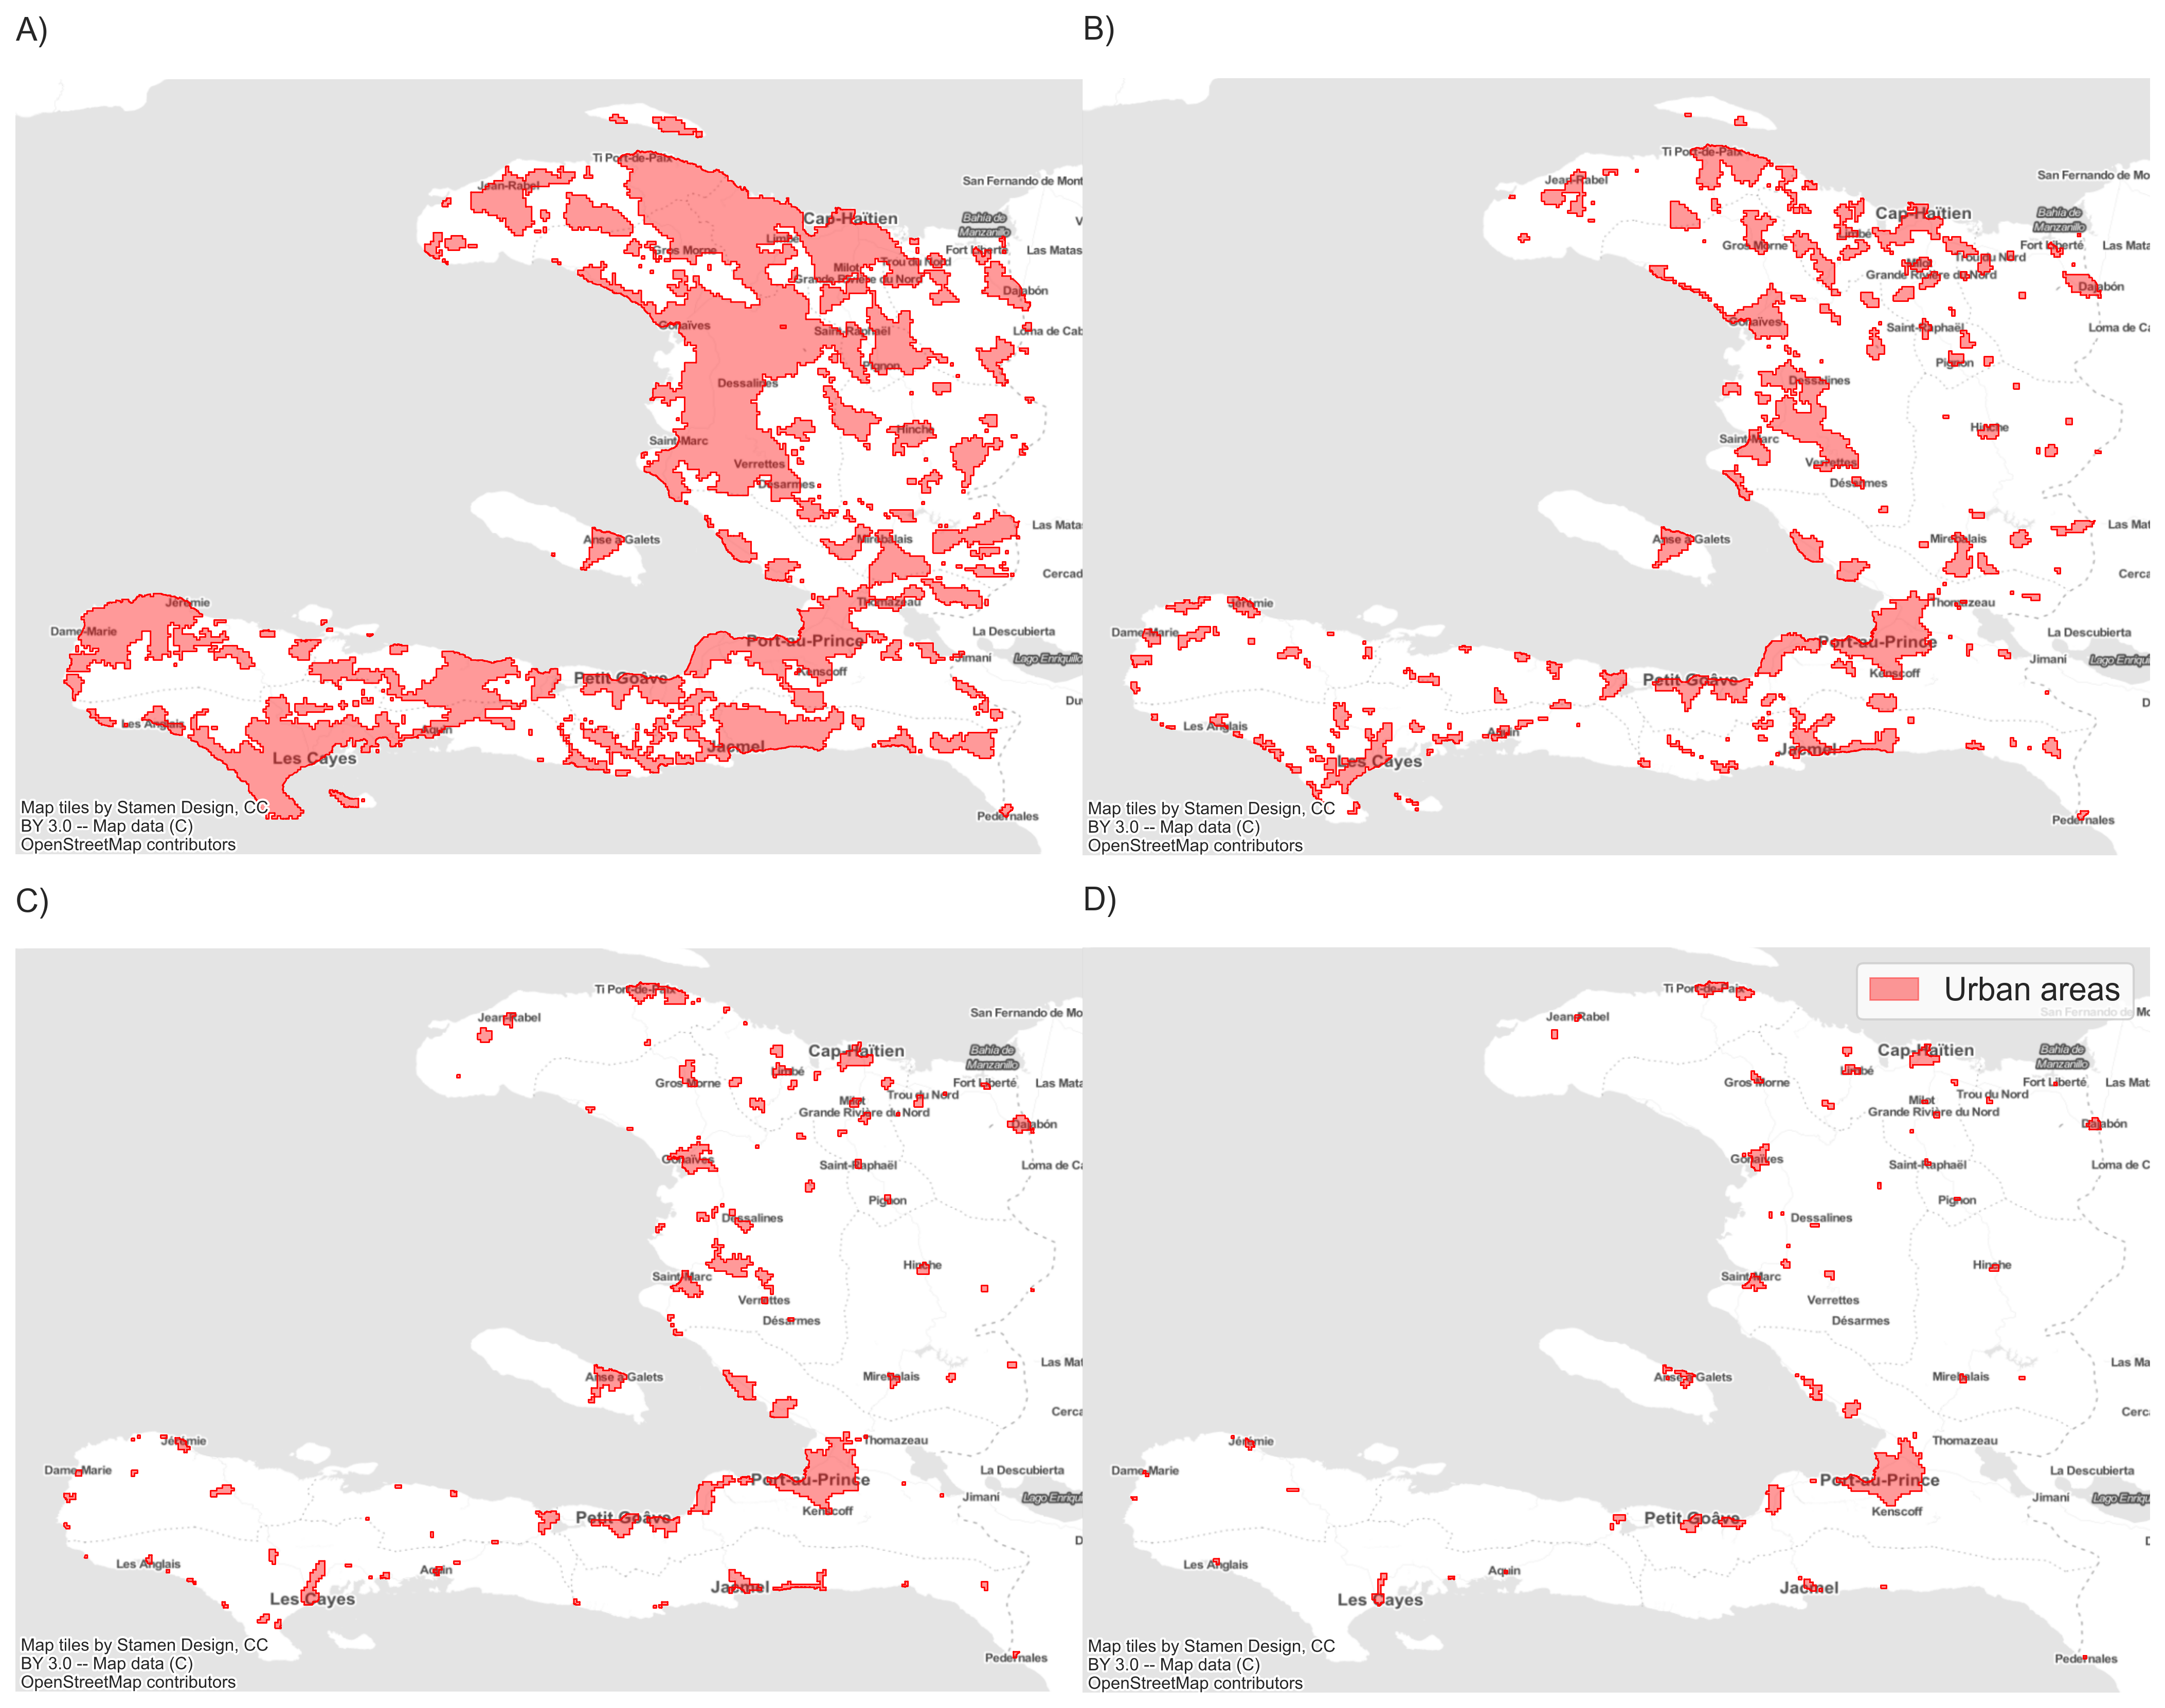
\includegraphics[width=\textwidth]{density_thresholds_haiti}
		\caption{Identified urban areas for Haiti, using the Worldpop dataset and several population density thresholds: (A) 200 (B) 400 (C) 800 (D) 1600 prs/km$^2$}
		\label{fig:hti_worldpop_explain_method}
	\end{figure}
	
	When considering the impact of each successive population density threshold on urban shapes, the relationship is more complicated.
	The Haiti case study suggests that higher density thresholds change the shapes of urban areas from more complex ones, to more compact urban area shapes.
	In the case of Haiti, a large proportion of urban areas are coastal and those urban boundaries bordering coastlines are spatially constrained.
	Since urbanization in coastal urban areas is generally driven by demand for closeness to coastlines, this coastline constraint results in more elongated shapes of coastal urban areas.
	When higher density thresholds are used for urban classification, large and elongated urban areas are spatially fragmented into a series of smaller urban areas.
	Spatial fragmentation first takes place for grid cells with the lowest population density.
	This includes coastal headlands, which generally have lower population densities, due to the higher friction of distance and lower accessibility to urban areas.
	Overall, the shapes of coastal urban areas are transformed from complex to increasingly compact shapes at higher density thresholds.
	This also transforms the number of places classified as urban, which is explored further in terms of national urban area counts in Section \ref{S:nus}.
	This pattern is unique to coastal urban areas and in particular for Haiti. 
	Further work is required to better understand the relationship between urban criteria and GPD on the shapes of urban areas and structure of urban systems in several countries.
	
	\subsection{National urban shares}
	\label{S:nus}
	
	The first urban indicator we assess using combinations of urban criteria and GPD is national urban shares.
	As noted, population density thresholds were only considered for this indicator.
	In general, we found a negative relationship between national urban shares and population density thresholds for each case study, regardless of GPD (Figure \ref{fig:urban_share}).
	In other words, urban classifiers that apply higher population density thresholds classify fewer grid cells as urban, which yields lower national urban shares.
	This is because fewer grid cells and their population fulfil the density criteria, so are not considered urban.
	
	
	\pagebreak
	\begin{figure}[H]
		\includegraphics[width=\textwidth]{national_urban_shares_portrait}
		\caption{Calculated national urban shares using population density thresholds only and each gridded population dataset for each country}
		\label{fig:urban_share}
	\end{figure}
	
	\pagebreak
	
	With respect to each of the GPD, calculated national urban shares were generally highest using the EU GHS-POP dataset (Figure \ref{fig:urban_share}).
	Comparatively, the GPW and WorldPop datasets were more similar, with the GPW generally reporting the lowest national urban shares.
	This general pattern was clearest for the countries of Rwanda, India and Indonesia but for other countries, including South Africa and Mexico, differences in calculated national urban shares between GPDs were small.
	Since the calculated national urban shares for South Africa and Mexico were more consistent for each GPD, this suggests that in these cases, the choice of urban criteria is more important than the choice of GPD. 
	Interestingly, calculated national urban shares were higher using the GPW and lowest for the GHS-POP for the United Kingdom and United States.
	This was also true for South Africa and Mexico but only for the highest density thresholds considered.
	This does suggest that there the choice of urban criteria and GPD could be influenced by a country's level of income.
	Therefore comparative urban analysis using rigid urban criteria may not be appropriate but given the small study sample, these results are not conclusive and future work should be considered at the global scale.
	
	We also compared the calculated national urban shares against estimates for the UN and newly adopted DEGURBA methodology (Figure \ref{fig:urban_share}).
	In general, we found that the DEGURBA reports a higher national urban share when compared to UN estimates.
	Furthermore, estimated national urban shares by the DEGURBA were only consistent with our approach when we applied the EU's own GHS-POP dataset.
	Conversely, the nationally reported urban shares using the previous UN definition was more consistent using the GPW and WorldPop datasets. 
	This not only highlights how the choice of GPD can change calculated urban indicators but also the uncertainties within the GPD themselves. 
	
	
	
	\subsection{National urban settlement counts}
	\label{S:nusc}
	National urban area counts were calculated using both a population density and count threshold for each GPD.
	We also found a negative relationship between national urban area counts and population density thresholds (Figure \ref{fig:settlement_relplot}).
	However, urban area counts did not consistently decrease, and at some density thresholds they actually increased.
	Here, large  areas are spatially fragmented into a series of small urban areas, as discussed in Section \ref{S:urban_shapes}.
	When evaluating the full range of density and population count thresholds, the spatial fragmentation process takes place at different density thresholds, whereas higher population count thresholds flatten the relative decrease in urban area counts.
	So how we classify and measure will have a direct bearing on our statistical interpretation of urban structure.
	
	
	\begin{figure}[H]
		\includegraphics[width=\textwidth]{national_urban_area_counts_portrait}
		\caption{Calculated national urban area counts (absolute) using both population density \& count thresholds and each gridded population dataset for each country}
		\label{fig:settlement_relplot}
	\end{figure}
	
	
	\pagebreak
	
	
	When calculating national urban area counts, the choice of GPD was generally more important than the choice of population density and count thresholds (Figure \ref{fig:settlement_relplot}).
	Similar to the calculated national urban shares, there were more urban areas using the GHS-POP dataset and considerably fewer count for the GPW dataset.
	This is related to the interpolation methods adopted by each GPD, whereby the population counts are considerably more spatially smoothed using the GPW dataset.
	Whilst this results in fewer urban areas being classified, this means that the total land area classified as urban is greater using the GPW. 
	However, the choice of population density and count thresholds were still important.
	Similar to the calculated national urban shares, we find the same reversal pattern exists in the importance of each GPD by level of income.
	Whereas calculated national urban settlement counts were generally the greatest using EU's GHS-POP dataset for low-income countries, urban area counts were actually higher using the GPW for high income countries.
	Nevertheless, we also find that calculated urban area counts for high-income countries are also stratified by population count thresholds first and then GPD.
	Conversely, urban area counts are generally stratified only by GPD for low-income countries. 
	Overall, calculated urban area counts in higher income countries appear to be strongly influenced by the choice of both GPD and population count threshold but population density thresholds are still important.
	
	
	By aggregating countries by level of income, the relationship between national urban area counts and income group are clearer (Figure \ref{fig:settlement_income_violinplot}).
	Interestingly, the interquartile range of area counts was generally highest using the GPW and lowest for the GHS-POP.
	However, the interquartile range was the highest using the GPW for high income countries.
	This again highlights the often overlooked uncertainties in the use of GPD and the need to carefully consider the choice of GPD for international statistical comparability.  
	However, this paper only assesses and compares key urban indicators using a small sample of countries, and because of this, these relationships may reverse in other samples.
	Future work should undertake this comparative analysis at the global scale.
	Overall, by comparing key urban indicators using our flexible approach to urban classification, we have shown that both the choice of urban criteria and GPD matters for comparing key international statistics.
	
	
	\begin{figure}[H]
		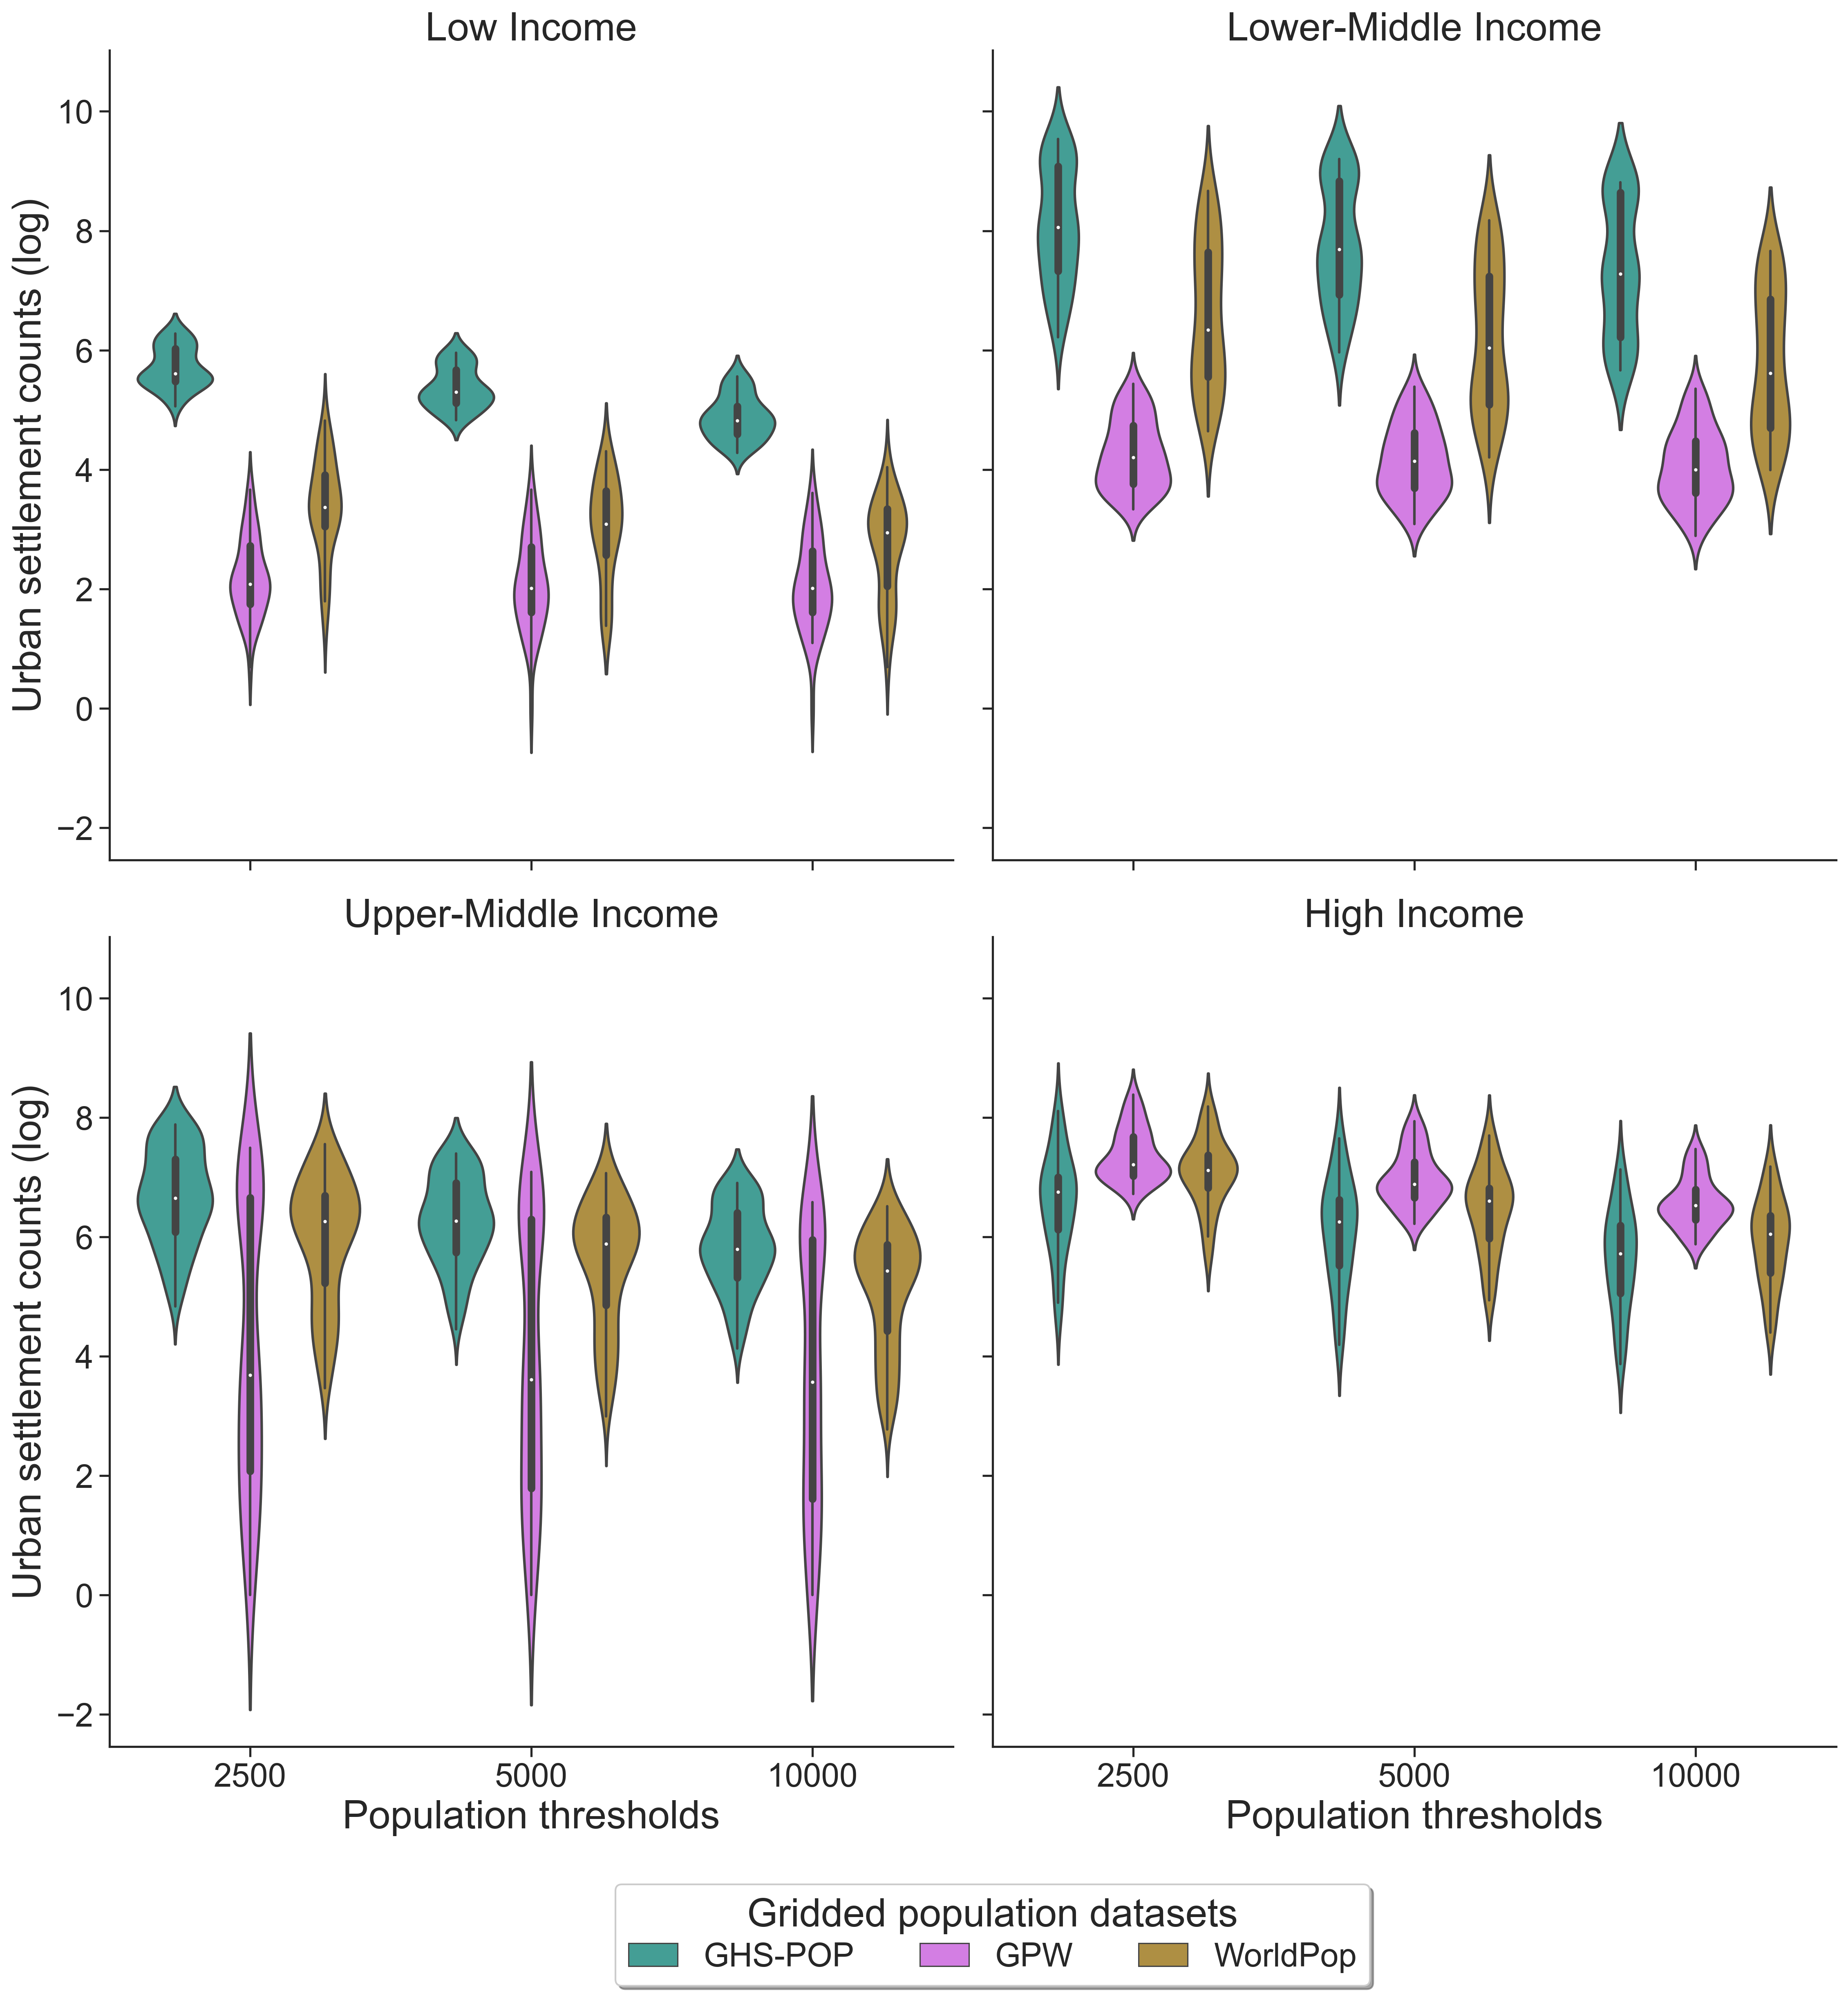
\includegraphics[width=\textwidth]{national_urban_area_counts_income}
		\caption{National urban area counts (relative) calculated for all population density thresholds and population count thresholds for each income group}
		\label{fig:settlement_income_violinplot}
	\end{figure}
	
	
	\section{Discussion and conclusions}
	This paper provides an alternative methodological approach to the recently agreed upon UN DEGURBA for urban classification and identification of urban areas.
	Prior to this agreement, international comparability of key urban statistics, including levels of urbanisation, was undermined by the fact different countries use different criteria for classifying urban and rural areas.
	Whilst the DEGURBA offers a standardised methodology for distinguishing between urban and rural areas, facilitating  international statistical comparability, the rigid criteria used for urban classification has been proven controversial.
	Instead of applying strict urban criteria for classification, our approach considers a range of population density and count thresholds.
	We also apply these rules to several GPD, to highlight the overlooked uncertainties when applying different GPD.
	To assess differences between urban criteria and GPD when applied to key urban indicators, we calculated and compared national urban shares and urban area counts for several countries.
	
	
	In general, we find an expected decrease in both calculated national urban shares and urban area counts using urban criteria with higher population density and count thresholds.
	In the case of national urban shares, we found that the proportion of the population classified as urban decreased at each higher density threshold considered but this decrease was much lower for higher density thresholds.
	Related to this, differences between GPD for calculated national urban shares were lower at higher density thresholds for urban classification.
	With higher density thresholds, more grid cells are classified as rural and fewer small settlements are classified as urban.
	This suggests that larger urban areas are less sensitive to the choice of density threshold and therefore, the choice of density thresholds is not as critical when classifying urban areas compared to smaller urban areas.
	These results are consistent with the literature, where definitions of large urban areas are more consistent compared to small-medium urban areas.

	
	When we considered both population density and count thresholds for calculated urban area counts, the number of urban areas did not decrease at higher density threshold.
	When both urban criteria were considered, large urban areas are spatially fragmented into smaller urban areas at certain density thresholds.
	These large urban areas are spatially fragmented either because the individual urban grid cells do not meet the density threshold, the total population count of each urban area does not meet the count threshold, or a combination of the two.
	However, when we considered even higher density thresholds, those spatially fragmented urban areas no longer met the next threshold requirements to be considered urban.
	This means that both total land area covered by urban areas and urban area counts then continued to decrease.
	
	
	Regardless of urban classification criteria, we found that the choice of GPD influenced both urban indicators.
	In general, both national urban shares and urban area counts were considerably higher using the EU GHS-POP dataset.
	The GPW and WorldPop datasets were much more consistent, with the GPW reporting the lowest national urban shares and urban area counts. 
	We also found that differences in both calculated urban indicators were highest for the low income countries.
	This may relate to the fact census enumeration errors vary spatially, where national statistical offices in higher income countries generally conduct more regular censuses, with known population distributions for spatially smaller statistical geographies or sources.
	Interpolating from sources to targets with spatial zoning systems that are closely matched in size and shape will likely introduce fewer errors.
	Given sources are generally spatially smaller in high income countries, interpolated errors are less likely using the same targets as for low-income countries.
	
	
	Of the GPDs, the GPW applies the simplest areal interpolation method, areal weighting, which relies on the area of overlapping geometries between sources and targets. 
	This results in spatially smooth interpolated population counts, where any errors correspond solely to these geometric properties.
	The other two approaches incorporate ancillary data to refine the areal interpolation but the GHS-POP also masks non-built up areas.
	The WorldPop method does not mask non-built up areas, leaving some residual population in areas that are not built up.
	This means that the WorldPop smooths population counts across both rural and urban areas. 
	This is based on the assumption that built-up area datasets don’t always accurately identify all populated areas. 
	Therefore, the population distribution for the WorldPop dataset is spatially smoother than the GHS-POP but not as spatially smooth as the GPW dataset. 
	Overall, this may explain why calculated urban indicators were much more consistent using the GPW and WorldPop datasets.
	
	
	Our alternative methodological approach has highlighted the uncertainties when selecting rigid urban criteria and single GPD for international statistical comparisons.
	We believe our approach offers a more flexible way for calculating key international statistical comparisons, compared to the rigid urban criteria adopted by the EU's DEGURBA.
	Whilst we only assessed our alternative approach using two key urban indicators, our approach has the capacity to inform urban policy from multiple standpoints.
	Future work should validate the findings in this study at the global scale, in addition to the refinement of GPDs more generally.
	
	\newpage
	
	\bibliography{references}
	
\end{document}